% !TeX spellcheck = en_US
\newpage
\section{Network}
The idea behind the network layer is to \textbf{interconnect} all the LANs, MANs and WANs. To do that it's necessary to introduce uniform internetwork addresses in an end-to-end packet format, abstracting the lower layers and creating a common format that's \textbf{independent} of intermediate link layer technologies.\\
This brings also the necessity to do:
\begin{itemize}
	\item \textbf{Routing}: automatically acquiring and updating next hop information for each destination
	\item \textbf{Forwarding}: moving incoming packets from the input interface to the appropriate output
\end{itemize}

\noindent The main \textbf{goal} of the network layer is to manage end-to-end connectivity across multiple networks. To do that it defines:
\begin{itemize}
	\item Internetwork identifiers
	\item Uniform end-to-end packet
	\item Routing and forwarding mechanisms
\end{itemize}
\begin{center}
	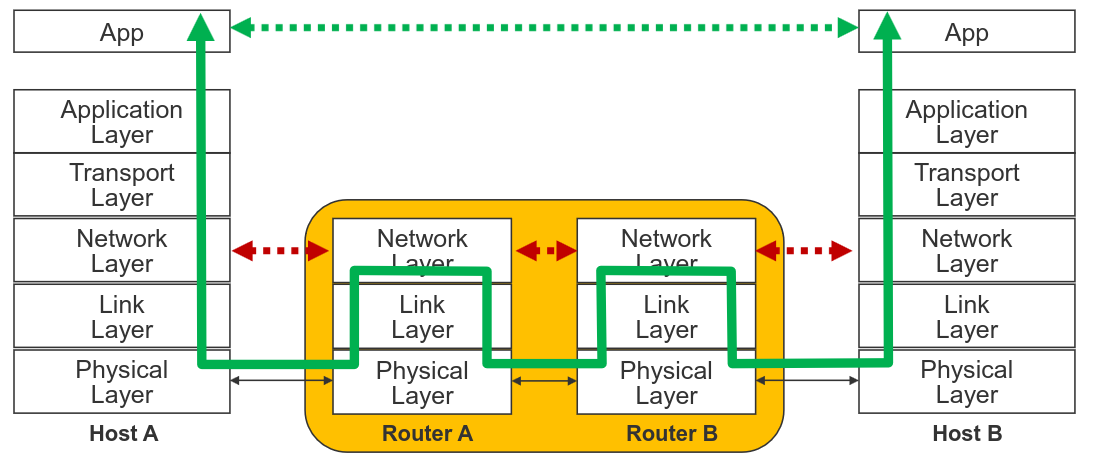
\includegraphics[scale=.3]{network}
\end{center}

\noindent There are two philosophies for \textbf{end-to-end connectivity}:
\begin{itemize}
	\item Connection-\textbf{less}: data is chunked and transferred as packets of variable length, with source and destination addresses in each one. Sending is made spontaneous without reservation. It's easy to implement but brings more challenges (wrong order of packets, delays, unreliability).
	\item Connection-\textbf{oriented}, with three phases:
	\begin{itemize}
		\item \textit{Connection establishment}
		\item \textit{Data transmission}: information exchange between the partners
		\item \textit{Connection termination}: release of the terminals and the channels
	\end{itemize}
	It's more complex to implement but brings reservation of capacity, flow control and no problem with sequence numbering.
\end{itemize}

\noindent Intermediate nodes need to \textbf{acquire} and \textbf{maintain} the \textbf{state} to establish paths, scope broadcasts and guarantee service quality. At the same time they need to handle \textbf{constraints}:
\begin{itemize}
	\item \textbf{Limited memory}: they cannot store an arbitrary amount of data
	\item \textbf{Limited throughput}: they cannot rely on an arbitrary amounts of control traffic to acquire the state
	\item \textbf{Limited computing capacity} and \textbf{speed}: they cannot compute arbitrary complex operations
\end{itemize}

\newpage
\subsection{Addressing}
Addresses are used to \textbf{identify} end hosts in multi-access networks and, in case of multi-address hosts, they help to select the right interface. They require:
\begin{itemize}
	\item \textbf{Compactness} of representation
	\item \textbf{Independence} from lower layers
	\item Built-in support for efficient and decentralized \textbf{path finding}
	\item \textbf{Uniqueness} within a network scope
\end{itemize}

\paragraph{Aggregation} Aggregation leads to much smaller intermediate states in intermediate nodes. Some example are:
\begin{itemize}
	\item \textbf{Geographical}: aggregate based on geographical area with a strict assignment policy
	\item \textbf{Hierarchical}: aggregate by organizations and sub-organizations, has a higher flexibility in assignment but may lead to less compression:
	\begin{itemize}
		\item \textit{Allocation}: initially a range of continuous addresses (determined by \textbf{prefix}) is given to an organization, which then can recursively delegate authority over parts of it. At the top the \textbf{Internet Assigned Numbers Authority} delegates to the \textbf{Regional Internet Registry} (AfriNIC, APNIC, ARIN, LACNIC and RIPE). They then delegate to \textbf{Local Internet Registry}, which are mostly ISP, enterprises or academic institution. They in the end assign IP to customers
		\item \textit{Assignment}: give an address to a host/interface
		\item \textit{Match}: longest common prefix match (match on prefix length), basically forward data to the output interface that shares more digits with the destination
	\end{itemize}
\end{itemize}

\paragraph{Challenges} The main challenges are:
\begin{itemize}
	\item \textbf{Security}: e.g. address spoofing when an attacker claims to own a network address of someone else since there is no global database
	\item \textbf{Efficiency}: effective aggregation requires careful address planning (keep large ranges, give unused addresses back)
	\item \textbf{Automation}: e.g. auto-configuration of address segment
\end{itemize}

\subsubsection{IPv4}
An IPv4 address is made of $4$ bytes divided in \textbf{network} part and \textbf{host} part. They can be:
\begin{itemize}
	\item \textbf{Public}: needs to be \textbf{unique}, typically one for each node
	\item \textbf{Private}: not unique and thus not globally routable.
\end{itemize}
\textit{Router} or \textit{gateways} usually have an IP address for each network they are linked to.
\begin{center}
	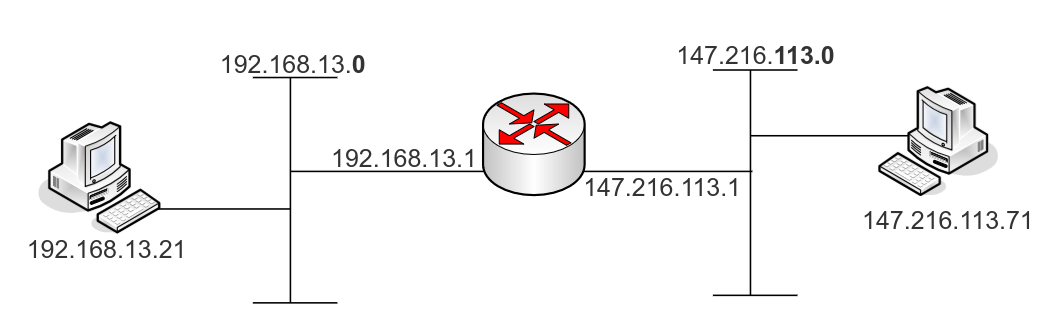
\includegraphics[scale=.3]{ipv4ex}
\end{center}

\paragraph{Classes}
\begin{wrapfigure}[5]{r}{5cm}
	\vspace{-0.5cm}
	\begin{center}
		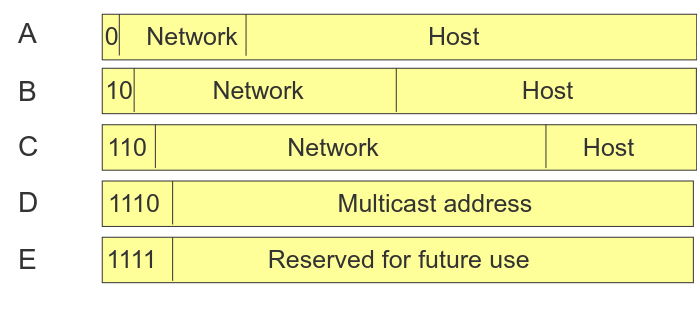
\includegraphics[width=5cm]{classes}
	\end{center}
\end{wrapfigure}
IP addresses are divided in five classes based on the first bits values. \\\\
Since nobody expected such an explosive growth of the internet, too many class A addresses were given away. Furthermore, class C networks are very small while class B are often too large.

\paragraph{Variable-Length Subnet Masking} To solve the problems of IP addresses, VLSM was introduced: static classes were replaced by network prefixes of any length.\\
Now an address is in the form $a.b.c.d/n$ where the first $n$ bits are the \textbf{network} identification and the remaining $32-n$ are the \textbf{host} identification. Another notation is the address and the explicit netmask in the form $u.x.y.z$.

\begin{note}
	VLSM is at the base of \textbf{Classless Inter-Domain Routing}.
\end{note}

\begin{definition}[Subnet]
	A subnet is a subset of addresses in a class A,B or C network. The principle is that some bits of the host addresses part are used to complement the network ID.
\end{definition}
All hosts on the same physical network use the same subnet mask. Combining IP address and subnet mask, a router determines to which subnet a packet must be sent.

\begin{center}
	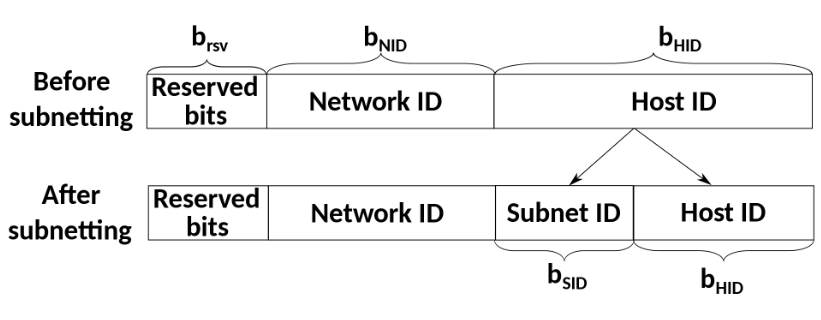
\includegraphics[scale=.3]{subnet}
\end{center}

\subsubsection{IPv6}
In 2011 IANA gives the last available blocks of IPv4 addresses. An extension was needed, hence the creation of IPv6: 128 bits divided in 8 couples of octets (8 bits).

\begin{note}
	IPv6 syntax allows to remove \textbf{leading zeros} in each one of the eight blocks and \textbf{replace} consecutive blocks of zeros with "::".
\end{note}

An IPv6 address is divided in three sections:
\begin{center}
	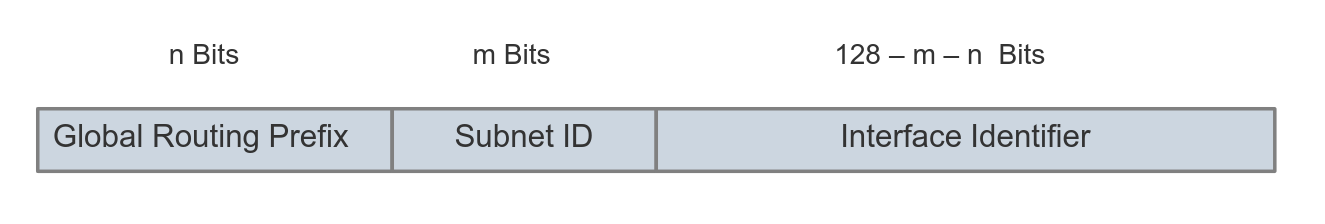
\includegraphics[scale=.3]{ipv6}
\end{center}
\begin{itemize}
	\item \textbf{Global Routing Prefix}: depends on RIR policy, for RIPE LIRs get /32 and ISPs get /48
	\item \textbf{Subnet Id}: assigned by network administrator
	\item \textbf{Interface identifier}: hash value identifying the NIC
\end{itemize}
\newpage
\noindent There are different types of addresses:
\begin{itemize}
	\item \textbf{Unicast}
	\begin{itemize}
		\item \textbf{Unique Local} $FC00::/7$
		\item \textbf{Link Local} $FE80::/10$
		\item \textit{IPv4-mapped} $::FF:0.0.0.0/96$
		\item \textit{Loopback} $::1/128$
		\item \textit{Unspecified} $::/128$
		\item \textbf{Global}: every other one
	\end{itemize}
	\item \textbf{Multicast} $FF00::/8$, it's an identifier for a group of interfaces. It has the following format:
	\begin{center}
		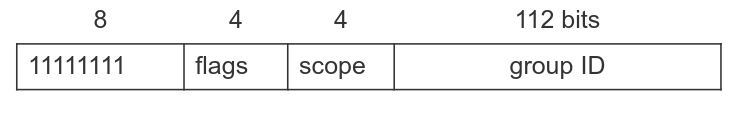
\includegraphics[scale=.3]{multicast}
	\end{center}
	\begin{itemize}
		\item \textbf{Flags}: 4 bits (0RPT) divided in:
		\begin{itemize}
			\item \textit{T}: if $1$, non permanently assigned (dynamically, on-demand), $0$ otherwise
			\item \textit{P}: multicast address assignment based on network prefix
			\item \textit{R}: embedding of the rendezvous point
		\end{itemize}
		\item \textbf{Scope}: defines the scope of the multicast
		\begin{table}[!h]
			\centering
			\begin{tabular}{c|c}
				\textbf{Value} & \textbf{Scope} \\
				\hline
				0 & Reserved \\
				1 & Interface-Local \\
				2 & Link-Local \\
				3 & Reserved \\
				4 & Admin-Local \\
				5 & Site-Local \\
				6, 7 & Unassigned \\
				8 & Organization-Local \\
				9-D & Unassigned \\
				E & Global scope \\
				F & Reserved
			\end{tabular}
		\end{table}
	\end{itemize}
	\item \textbf{Anycast}: chosen from unicast range and can be used to identify the router in a subnet, an organization or in a particular routing domain. It has the following format:
	\begin{center}
		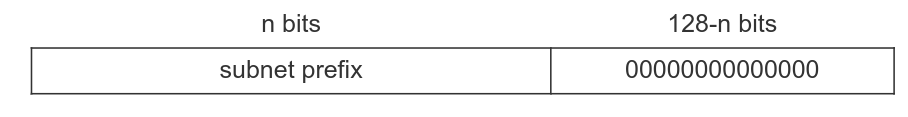
\includegraphics[scale=.3]{anycast}
	\end{center}
	\item \textbf{Broadcast}: dropped, use multicast
\end{itemize}

\newpage
\subsection{Internet Protocol}
Designing a protocol that serves the need for more than 40 years of technological development is really non-trivial since there is a continuous change of the upper- and lower-layer technologies.\\
Internet Protocol version 4 is the fundamental network layer protocol of the current Internet. The basic \textbf{properties} are:
\begin{itemize}
	\item \textbf{Transparent end-to-end communication} between hosts
	\item \textbf{Connectionless} and \textbf{packet-oriented}
	\item \textbf{Unreliable}, it provides a best-effort service
	\item \textbf{Hierarchical addressing}
	\item Support of \textbf{packet fragmentation}
\end{itemize}

\subsubsection{IPv4}
The IPv4 packet has the following format:
\begin{center}
	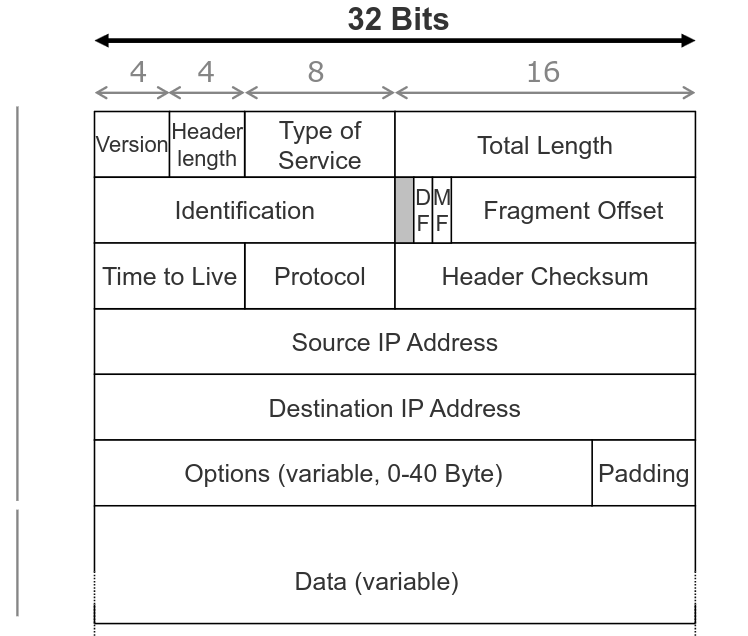
\includegraphics[scale=.3]{ipv4format}
\end{center}
\begin{itemize}
	\item \textbf{version}: either $4$ for IPv4 or $6$
	\item \textbf{length}: usually $20$ bytes but depends on the IP options
	\item \textbf{type of service}: allows different packets to be treated differently (e.g. low delay for voice, high bandwidth for video). Today it's used for \textbf{Differentiated Service Code Point} and \textbf{Explicit Congestion Notification}
	
	\paragraph{DSCP} This protocol is the introduction of \textbf{QoS} in IP network instead of best-effort. It uses a 6 bit flag and supports different types of services (e.g. video, voice). It defines various \textbf{Per-Hop Behaviors} that set the packet forwarding properties for a class of traffic:
	\begin{itemize}
		\item \textbf{Default}: best-effort traffic
		\item \textbf{Expedited}: loss-low, low-latency traffic
		\item \textbf{Assured}: assurance of delivery under prescribed conditions
		\item \textbf{Class Selector}: maintain backward compatibility with the old IP field
	\end{itemize}
	It introduces the principle of \textbf{traffic classification}, where each data packet is classified into one of a limited number of classes. Each router is then configured to differentiate traffic based on its class.
	
	\item \textbf{total length}: number of bytes of the entire packet, the maximum being $2^{16}-1$ bytes
	
	\paragraph{Fragmentation} Every link on the internet has a \textbf{Maximum Transmission Unit}, the number of bytes a link can carry as one unit. If the outgoing MTU is smaller than the total packet size, a router can \textbf{fragment} a packet, which are then recomposed at destination.
	
	\item \textbf{identification}: all fragments belonging to the same packet have this same value
	\item \textbf{More Fragments}: a single bit which indicates if this is the last fragment of a datagram $0$ or if further will follow $1$
	\item \textbf{Don't Fragment}: all router must forward packets up to a size of $576$ bytes, everything beyond that is optional. Larger packets with this bit set to $1$ might be discarded
	\item \textbf{fragment offset}: it's the position of a packet a fragment belongs to, counted in multiples of $8$ bytes
	\item \textbf{Time To Live}: it's used to limit packet travel time and identify and mitigate loops. Its value is decremented by $1$ at each router it passes and it's discarded when it reaches $0$
	\item \textbf{protocol}: identifies the higher-level protocol, such as TCP or UDP
	\item \textbf{header checksum}: it's the sum of all $16$ bits words in the header
	\item \textbf{source IP address}
	\item \textbf{destination IP address}
	\item \textbf{options}: were initially put to provide additional flexibility but now for security reasons are often deactivated since they could reveal information
\end{itemize}

\subsubsection{IPv6}
IPv6 was implemented first of all to have more addresses. But that was not the only reason:
\begin{itemize}
	\item Simpler \textbf{addressing} and \textbf{routing}
	\item Simpler \textbf{protocol architecture}: slim fixed header, optional extensions, format framework for header classes, no header checksum (done in other layers) and no fragmentation
	\item Simpler \textbf{administration}: auto-configuration of interfaces without DHCPv6 and renumbering via prefix change
	\item Additional \textbf{security}, improved multicast, anycast, \textbf{QoS}, support of \textbf{Jumbograms}
\end{itemize}

\paragraph{History} IP next generation work began in the early 90s: in 1992 there were several proposal for the development of IP. After several merges in 1993 \textbf{Simple Internet Protocol Plus} and \textbf{Common Architecture for the Internet} were created. In 1994, SIPP was chosen.\\
In 1995 the IPv6 specification rolled out and in 1999 user addresses were available. \\
In May 2007 ARIN advises the beginning of IPv6 migration and in 2012 there is the world launch.

\paragraph{Packet} The packet is formatted as follows:
\begin{center}
	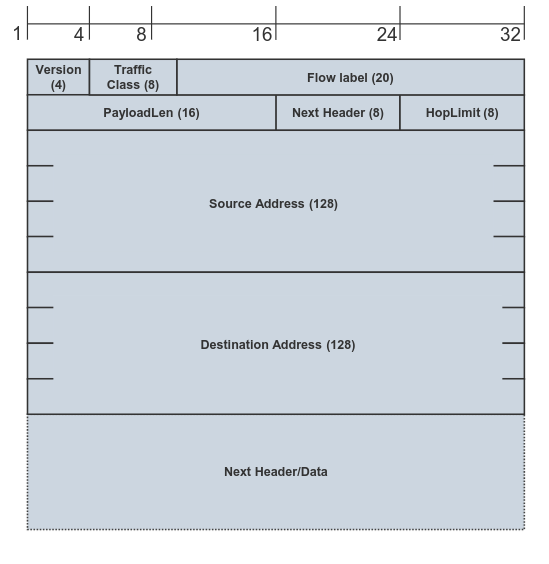
\includegraphics[scale=.28]{ipv6format}
\end{center}

\begin{itemize}
	\item \textbf{version}: IP version number
	\item \textbf{traffic class}: classifying packets
	\item \textbf{flow label}: virtual connection with certain characteristics or requirements
	\item \textbf{payloadLen}: packet length after the 40 bytes header
	\item \textbf{nextHeader}: indicates the type of the following extension header or the transport header
	\item \textbf{hopLimit}: decremented by one at each hop, if zero discarded
	\item \textbf{source address}
	\item \textbf{destination address}, not necessary if there is an optional routing header
	\item \textbf{next header/data}, if an extension header is specified, it follows after the main header, otherwise the data are following
\end{itemize}

\paragraph{Comparison} The IPv6 header is longer than the IPv4 but it's only because of the longer addresses. Otherwise, it's better sorted and thus \textbf{faster} to process by routers.\\
\textbf{Fragmentation} was removed, among with checksum and header length, to leave the problem to the end host and simplify the handling.

\paragraph{Extension headers} They extend basic IPv6 functionalities. Each header may either reference another extension or the data. The main extensions are:
\begin{itemize}
	\item \textbf{Routing}: definition of a full or partly specified route (deprecated since 2007)
	\item \textbf{Fragmentation}: same as IPv4 but now only the source can fragment and if a router finds a packet that's too big, an error is sent back
	\item \textbf{Authentication}: security information, authentication of the sender
	\item \textbf{Encapsulation}: tunneling e.g. for encrypted data
	\item \textbf{Hop-by-Hop options}: dedicated options to be processed by every router and host, at the moment only the Jumbogram implementation is supported
	\item \textbf{Destination options}: additional information for the destination
\end{itemize}

\paragraph{Options} For maximum flexibility, options are possible in headers. They have no length limit and are encoded as \textbf{Type-Length-Value}:
\begin{center}
	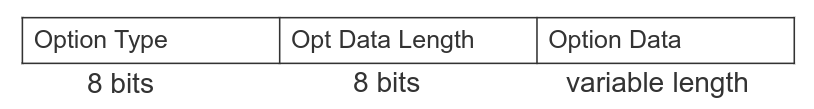
\includegraphics[scale=.3]{tlv}
\end{center}
The \textbf{Option Type} defines also:
\begin{center}
	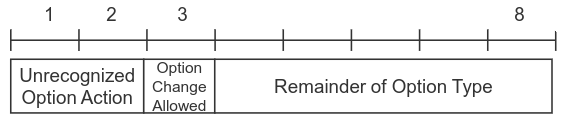
\includegraphics[scale=.3]{options}
\end{center}
\begin{itemize}
	\item \textbf{Unrecognized Option Action}: the action that must be taken if a node does not recognize the Option Type
	\begin{itemize}
		\item $00$: skip this option and continue with the rest
		\item $01$: discard the packet
		\item $10$: discard the packet and ICMP the source with \textit{unicast} and \textit{multicast}
		\item $11$: discard the packet and ICMP the source with \textit{unicast}
	\end{itemize}
	\item \textbf{Option Change Allowed}: indicates whether or not the \textbf{Option Data} can be modified while the datagram is en route
\end{itemize}

\begin{observation}[Length]
	IPv6 requires a minimum \textbf{MTU} of 1280 bytes. Links which cannot convey such big packets have to apply link-specific fragmentation and assembly at a layer below IPv6.
\end{observation}

\paragraph{Path MTU} It's the minimum link MTU of all the links in a path between a source node and a destination node. The originating node assumes that the PMTU is the MTU of the first hop. A \textbf{trial packet} of that size is sent out. If any link is unable to handle it, an ICMPv6 Packet \textbf{Too Big} is sent back and the originating node tries again with a smaller MTU.

\subsubsection{Migration}
IPv6 cannot be introduced overnight: for some time both variants will coexist. An \textbf{incremental deployment} is needed, which includes:
\begin{itemize}
	\item \textbf{Porting}: making applications IPv6 ready, which means using a new API
	\item \textbf{Migration}: done step by step through different techniques
	\begin{itemize}
		\item \textbf{Dual stack}: allowing the coexistence of both versions on the same device and subnet. The application chooses which one to use. It can continue indefinitely but means an increased use of IPv4 NAT.
		\begin{center}
			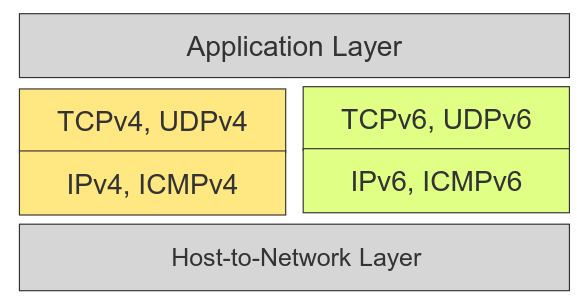
\includegraphics[scale=.2]{dualstack}
		\end{center}
		One of the main protocols is \textbf{Dual Stack Lite}: there is no IPv4 in the public internet, just in the private networks. IPv4 runs then over IPv6 and many customers can share a single globally unique IPv4 address.
		\item \textbf{Tunneling}: connecting IPv6 regions over IPv4 regions. Routers encapsulates incoming IPv6 packets into a new IPv4 one with destination address of the next router also supporting IPv6. There is more \textbf{overhead} but no data loss.The main techniques are:
		\begin{itemize}
			\item \textbf{6-over-4}: IPv6 islands in an IPv4 world with an IPv6 backbone. The end-user site network stuff must choose an IPv6 Internet Service to tunnel to or peer with other islands
			\item \textbf{6-to-4}: isolated IPv6 islands in an IPv4 world. It allows the islands to automatically interconnect, defining \textbf{point-to-multipoint tunnels} and assigning an IPv6 prefix to each IPv4 address (DNS will return both). Then the nearest router identifies 6to4 packet based on a special IPv6 prefix and encapsulates it in IPv4
		\end{itemize}
		\item \textbf{Protocol Translator} (NAT): let IPv6 devices speak to IPv4 ones
	\end{itemize}
\end{itemize}

\newpage
\subsection{Assignment and mapping}
\subsubsection{ARP}
The \textbf{Address Resolution Protocol} discovers the MAC addresses associated with an IP address, which is needed for the lower layers that do not understand IP.\\
Each host stores known IP and MAC addresses in a table: the \textbf{ARP cache}. The entries become invalid after a certain amount of time, to avoid mistakes. The entries are inserted through ARP \textbf{requests} (broadcasts) and \textbf{responses}. \\
To optimize the process, each computer occasionally sends an ARP request to it's own IP address. On some systems a host periodically sends out requests for each entry.\\
The packet format is designed to be used with various network and link layers by specifying the length:
\begin{center}
	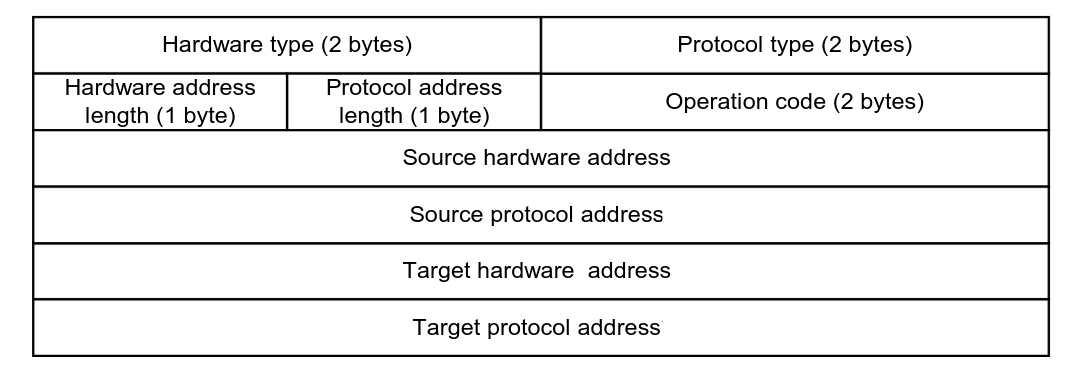
\includegraphics[scale=.3]{arp}
\end{center}

\paragraph{Risks} Since an ARP request-response is \textbf{stateless} and \textbf{not authenticated}, the ARP cache is updated every time it receives a reply, even if it didn't send out one. This creates risks for:
\begin{itemize}
	\item \textbf{Spoofing}: a rogue machine can spoof other machines by replying with wrong data
	\item \textbf{Cache poisoning}: a rogue machine can poison an ARP cache by sending forged ARP replies
\end{itemize}

\subsubsection{RARP}
The \textbf{Reverse} Address Resolution Protocol a computer can ask it's own IP address by sending out his MAC address. A RARP server then replies with the IP. Deprecated.

\subsubsection{DHCP}
\begin{wrapfigure}[10]{r}{8cm}
	\vspace{-1.5cm}
	\begin{center}
		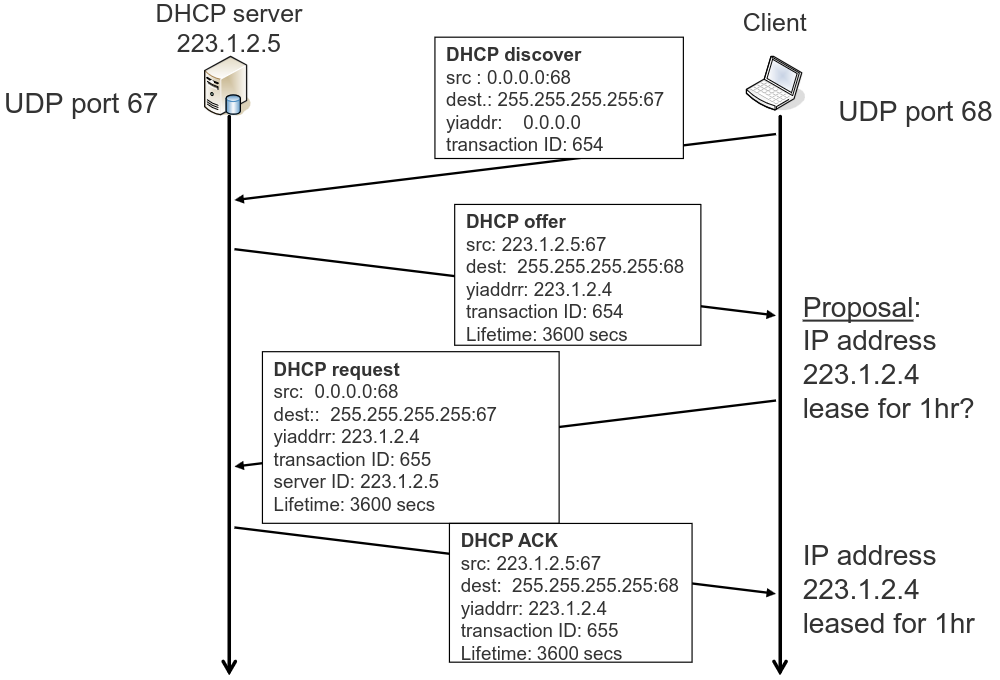
\includegraphics[width=7cm]{dhcp}
	\end{center}
\end{wrapfigure}
Since RARP requests are not passed on by routers, the computer sends out a DHCP packet. In each subnet there is also a \textbf{DHCP Relay Agent} which passes those messages to the DHCP server.\\
Furthermore, to communicate globally you need more than the IP address (subnet mask, defaul router, DNS server) and those are configured by the DHCP.\\
DHCP works in three phases:
\begin{itemize}
	\item \textbf{Service discovery}: the host does a \textbf{DHCP Discover} (broadcast), where he states his MAC address and asks for an IP one. The server then answers with a \textbf{DHCP Offer} (unicast) where he offers the IP address and other configurations (DHCPINFORM).
	\item \textbf{IP Address Assignment}: the host sends out a \textbf{DHCP Request} (broadcast) stating his MAC address and the IP address that he wants to use. The server sends out a \textbf{DHCP Ack} (unicast) to accept that (or NACK to deny).
	\item \textbf{Address release}: IP addresses may be permanently assigned or leased for a limited period of time. After the lease expiration you need to explicitly renew the lease or relinquish the address (\textbf{DHCPRELEASE})
\end{itemize}

The DHCP packet format was mostly inherited from a previous protocol (BOOTP) and its the following:
\begin{center}
	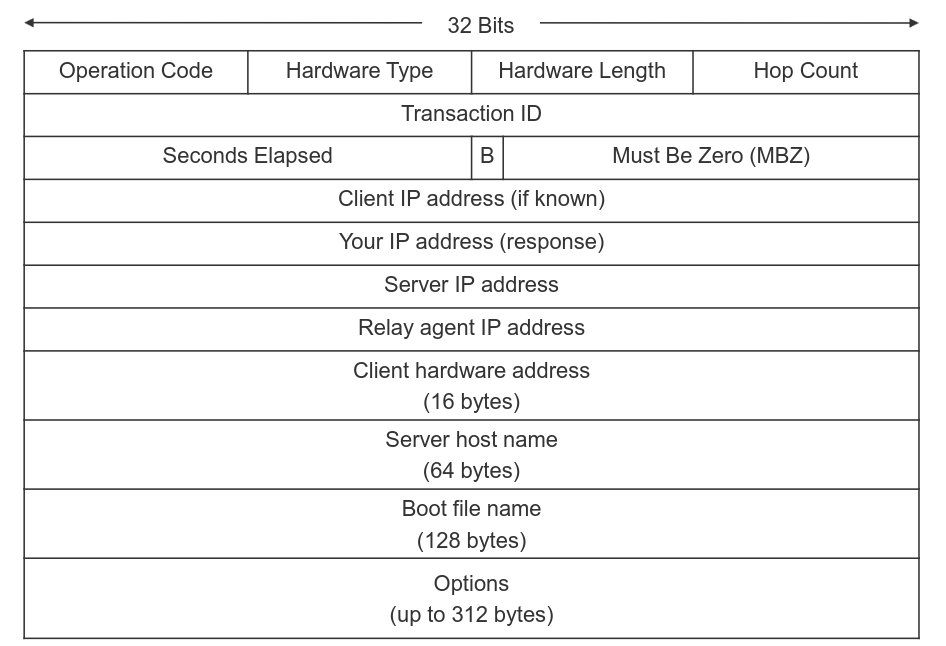
\includegraphics[scale=.3]{dhcpformat}
\end{center}

\begin{note}
	DHCP uses UDP and therefore is \textbf{unreliable}.
\end{note}

\subsubsection{NDP}
In IPv6 instead of ARP, \textbf{Network Discovery Protocol} is used. This protocol is also used for:
\begin{itemize}
	\item \textbf{Neighbor Unreachability Detection}
	\item IPv6 \textbf{address autoconfiguration}
	\item \textbf{Router discovery}
	\item \textbf{On-link prefix discovery}
	\item \textbf{Next-hop determination}
	\item \textbf{Link parameter discovery}, e.g. MTU
	\item \textbf{Redirect}: indicate better next-hop
	\item \textbf{Duplicate Address Detection}
\end{itemize}

\noindent The packet format is a classic ICMPv6 one:
\begin{center}
	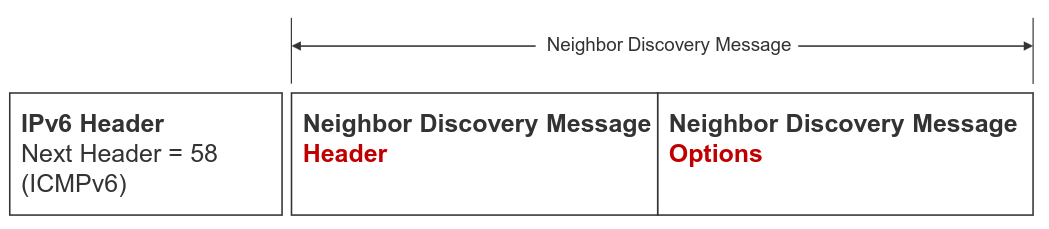
\includegraphics[scale=.3]{ndp}
\end{center}
The possible operations are, compared to IPv4:
\begin{table}[!h]
	\centering
	\begin{tabular}{|c|c|}
		\hline
		\textbf{IPv6} & \textbf{IPv4} \\
		\hline
		\textit{Neighbor Solicitation} & ARP Request \\
		\hline
		\textit{Neighbor Advertisement} & ARP Reply \\
		\hline
		\textit{Neighbor Cache} & ARP Cache \\
		\hline
		\textit{Router Solicitation}& Router Solicitation \\
		\hline
		\textit{Router Advertisement} & Router Advertisement \\
		\hline
		\textit{Redirect Message} & Redirect Message\\
		\hline
	\end{tabular}
\end{table}

\begin{note}
	One advantage of using NDP is that it's a pure network protocol contrary to ARP, meaning that one can also apply network layer security mechanisms solving problems like spoofing.
\end{note}

\subsubsection{SLAAC}
\textbf{State-Less Address Auto-Configuration} is the IPv6 stateless equivalent for DHCP. It's divided in three phases:
\begin{enumerate}
	\item \textbf{Acquire Link Local} IPv6 address: generate a tentative link-local based on the MAC address, used \textbf{Duplicate Address Detection} (send a \textit{Neighbor Solicitation} to that address): if the address exists, fail and go to manual, otherwise if there is no response, convert the \textbf{Extended Unique Identifier} 48 bits MAC into a EUI 64 bit dynamically assigned host identifier:
	\begin{enumerate}
		\item Leftmost 24 bit of the MAC form the leftmost 24 bits of the EUI-64
		\item Rightmost 24 bit of the MAC form the rightmost 24 bits of the EUI-64
		\item Insert the constant $FFFE$ in the middle
		\item Tweak left-most bit 7 from zero to one
		\item Prepend $FE80::$
	\end{enumerate}
	\item \textbf{Contact router}: once the link-local address is assigned to the interface, the node sends out a \textbf{router solicitation} to the well-known address $FF02::1$ (All Routers) and the router responds with a \textbf{Router Advertisement}
	\item \textbf{Configure Global IPv6 Addresses}: process the \textit{router advertisement} message that has been received, which includes the network ID prefix and two flags:
	\begin{itemize}
		\item \textbf{Managed Address Configuration}: if $1$, stop and do stateful configuration, otherwise assign the global IP Global IP:Host ID/64 and check the other flag
		\item \textbf{Other Stateful Configuration}: if $0$, stop, otherwise use stateful configuration for other information such as name server
	\end{itemize}
\end{enumerate}